\RequirePackage{plautopatch}
% 一応pLaTeX用パッチを当てておく
% クラスオプションでdvipdfmxを読み込めばusepackageで個別に指定する必要がなくなる
% jarticleは非推奨なので使いたくないが、レギュレーションなので大変遺憾に思いつつ従う
\documentclass[dvipdfmx,12pt,a4j]{jarticle}
% dvipdfmxはグローバルオプションとして読み込んでいるので個別のパッケージのオプションとしては不要
\usepackage{graphicx}
% ロゴ関係
\usepackage{bxtexlogo}
\bxtexlogoimport{*,**}
% Hオプションを使いたいので読み込む
\usepackage{here}
% ソースコードを表示するのに読み込む
\usepackage{listings}
% シンタックスハイライトのため
\usepackage{xcolor}
% url挿入のため
\usepackage{url}
% xcolorの色定義
\definecolor{solarized@base03}{HTML}{002B36}
\definecolor{solarized@base02}{HTML}{073642}
\definecolor{solarized@base01}{HTML}{586e75}
\definecolor{solarized@base00}{HTML}{657b83}
\definecolor{solarized@base0}{HTML}{839496}
\definecolor{solarized@base1}{HTML}{93a1a1}
\definecolor{solarized@base2}{HTML}{EEE8D5}
\definecolor{solarized@base3}{HTML}{FDF6E3}
\definecolor{solarized@yellow}{HTML}{B58900}
\definecolor{solarized@orange}{HTML}{CB4B16}
\definecolor{solarized@red}{HTML}{DC322F}
\definecolor{solarized@magenta}{HTML}{D33682}
\definecolor{solarized@violet}{HTML}{6C71C4}
\definecolor{solarized@blue}{HTML}{268BD2}
\definecolor{solarized@cyan}{HTML}{2AA198}
\definecolor{solarized@green}{HTML}{859900}
% listingsのスタイル定義
\lstdefinestyle{c}{
  language=c,
  numbers=left
}
\lstset{
basicstyle=\small\ttfamily\color{solarized@base00},
rulesepcolor=\color{solarized@base03},
numberstyle=\scriptsize\color{solarized@base01},
keywordstyle=\color{solarized@blue},
stringstyle=\color{solarized@cyan}\ttfamily,
commentstyle=\color{solarized@base01},
emphstyle=\color{solarized@red},
backgroundcolor=\color{solarized@base3},
sensitive=true,
breaklines=true,
breakatwhitespace=true,
framerule=0pt,
frame=l
showstringspaces=false,
tabsize=2,
basewidth={0.57em,0.52em},
}
\title{プログラミング 第1回レポート}
\author{202111609 仲村和士}
\date{\today}

\begin{document}
\maketitle
\section{はじめに}
課題内容を始める前に重要なことを何点かこの節で述べる。

\subsection{\BibTeX のコンパイルについて(重要)}
はじめに本レポートをコンパイルする際の注意点について述べたい。本レポートの文献情報には日本語書籍が含まれている。したがって通常の\BibTeX ではなく\pBibTeX を利用することを推奨する。
\begin{verbatim}
  $ pbibtex -kanji=utf-8 file_name
\end{verbatim}

\subsection{\LaTeX 利用の方針}
随時インターネットで調べた結果を活用するが、日本語\LaTeX の代表的書籍である、奥村、黒木~\cite{bibunsho}に記述があるものはこれに従う。講義資料と齟齬がある点についてはその都度記述する。

ただし、例外的にjarticleを利用する点のみ前述の書籍の記述から外れるものとする。\LaTeX の作法としては非推奨であるが、今回のレポートのレギュレーションである以上それに従うものとする。

\section{Linuxのコマンド利用}
\subsection{課題内容と方針}
本課題は講義ノートで扱ったコマンドを\LaTeX の表形式でまとめる課題である。講義ノートではLinuxのシェル利用の基礎知識\footnote{レポートを書く前に整理したところ、環境構築と導入、シェルの補完関係の機能、絶対パスと相対パス、テキストエディタ、パイプとリダイレクトなどが含まれる。これらも非常に大切であるが、レポートの設問意図からは外れると思われるため、あえて記述はしない。}なども多く書かれているが、本レポートでは設問の意図より、それらは省略してファイル操作コマンドを中心にまとめることとする。

講義ノートで出てきているコマンドはあまり多くないとはいえ、ただ順番に列挙しただけではあまり見やすくないし、表にする意味が薄れてしまう。そこで、コマンドを4つの系統に分けて整理することにした。以下の4つである。
\begin{enumerate}
  \item ファイルおよびディレクトリの情報確認とディレクトリの移動
  \item ファイルおよびディレクトリへの操作
  \item プログラムの中断と再開
  \item その他
\end{enumerate}

次の小節からはこれに沿って本文を構成する。また、表の出力にはtable環境およびtabular環境を利用する。表の構成はコマンド名、主要なオプション、機能、実行例とする。これに関しては私が昨年書いた情報科学特別演習の最終レポート内で類似のコマンドリストを作っているため、こちらも一部参考にした。

\subsection{情報確認とディレクトリの移動}
ここからは、実際にUNIXコマンドを用いてファイルおよびディレクトリの情報を確認する方法、およびディレクトリの移動方法を解説する。

まず、ファイルおよびディレクトリの基本的な情報を調べるときにはlsコマンドを用いる。lsコマンドは引数にパスを与えるとそのディレクトリに存在するファイル一覧を表示する。引数がないときにはカレントディレクトリの情報を表示する。与えられたパスがファイルのときはそのファイル自身の情報を表示する。よく使うオプションは-lと-aであり、-lオプションではより詳しい情報を表示する。-aではデフォルトでは非表示のdotfilesを表示する。

ファイルの中身を確認するときにはcatコマンドを使う。catコマンドは引数に取ったファイルの内容を標準出力へ出力する。引数がない時には、標準入力を受け取る。しかし、ファイルの内容が多く、一画面に収まらないときもある。そのようなときはlessコマンドを使う。lessコマンドは与えられたファイルの中身を一画面ずつ出力する。移動にはj,kで上下移動、qで終了といったvimライクなキーバインドが用いられる。

ファイルの行数、単語数、バイト数を確認するときにはwcコマンドを利用する。wcコマンドは引数にとったファイルの行数、単語数、バイト数を表示する。

カレントディレクトリを表示するときにはpwdコマンドを利用する。余談であるが、私は初学の頃にパスワードを設定するpasswdコマンドと混乱したので注意されたい。

カレントディレクトリを移動するときにはcdコマンドを使う。cdコマンドを使うと引数に与えたパスに移動する。パスの指定方法は絶対パスでも相対パスでもよい。引数なしでの実行は普通cd \verb|~| と等価であり、ホームディレクトリに移動する。また余談であるが、非常に便利なcd - というコマンドを紹介する。これを実行するとひとつ前にいたディレクトリに移動することができる。ひとつ前のディレクトリのみにしか移動できないので完全に代用することはできないが、意図的にスタックを操作する必要がないので類似の機能を提供するpushd/popdより手軽に利用できる。

表\ref{table:command:info}にここまでのコマンドをまとめた。
\begin{table}[H]
  \caption{コマンドまとめ: 情報確認とディレクトリ移動}
  \label{table:command:info}
  \begin{tabular}{|c|l|l|l|}
    \hline
    コマンド名 & 主要オプション & 機能 & 実行例\\
    \hline \hline
    ls & -l -a & ディレクトリにあるファイル情報を表示 & ls -la \\
    cat & & ファイルの中身を表示 & cat scheme.sql \\
    less & & ファイルの中身を1画面ずつ表示 & ps aux \verb+|+ less \\
    wc & & ファイルの行数、単語数、バイト数を表示 & ls -l \verb+|+ wc \\
    pwd & & カレントディレクトリを表示 & pwd \\
    cd & & カレントディレクトリを移動 & cd ..\\
    \hline
  \end{tabular}
\end{table}

\subsection{ファイルおよびディレクトリへの操作}
ファイルおよびディレクトリに対する操作を行う方法について説明する。

まず、空のファイルを作成するときにはtouchコマンドを用いる。touchコマンドは本来、引数にとったファイルのタイムスタンプを変更するためのコマンドであるが、引数にとったファイルが存在しない場合は新たに作成する。-cオプションを付けると、新規ファイル作成を行わない。

ファイルを削除するときにはrmコマンドを利用する。rmコマンドは引数にとったファイルを削除する。一度削除すると復元できないので注意が必要である。-rオプションを付けるとディレクトリ内を再帰的に削除することができる。

ファイルをコピーするときはcpコマンドを利用する。cp コピー元 コピー先 のように記述する。-rオプションをつけるとディレクトリ内を再帰的にコピーする。-iオプションを付けると上書きに対する警告をしてくれる。

ファイルを移動するときにはmvコマンドを利用する。書式はcpコマンドと同様である。-iオプションの挙動も同様である。mvコマンドはcpコマンドと異なり、削除の権限がないと利用できないのでシステム管理の際は注意を要する。

ディレクトリを作成するときにはmkdirコマンドを利用する。mkdir ディレクトリ名という形式で利用する。

ディレクトリを削除するときにはrmdirまたはrm -rを利用する。rmdirは空のディレクトリのみ削除できるのに対して、rm -rは中にファイルが入っていても再帰的に削除できる。

表\ref{table:command:file}にここまでのコマンドをまとめた。

\begin{table}[H]
  \caption{コマンドまとめ: ファイルおよびディレクトリへの操作}
  \label{table:command:file}
  \begin{tabular}{|c|l|l|l|}
    \hline
    コマンド名 & 主要オプション & 機能 & 実行例\\
    \hline \hline
    touch & -c & タイムスタンプの変更、ファイル作成 & touch a b c \\
    rm & -r -f & ファイルの削除 & rm a \\ 
    cp & -i -r & ファイルのコピー & cp a ./sub/a \\
    mv & -i & ファイルの移動、リネーム & mv ./sub/a x \\
    mkdir & & ディレクトリの作成 & mkdir /mnt \\
    rmdir & & ディレクトリの削除 & rmdir ./sub \\
    \hline
  \end{tabular}
\end{table}

\subsection{プログラムの中止と再開}
前面にあるプログラムの中止と再開に関するコマンドについて説明する。

前面で実行中のジョブは、C-zにより中断できる。中断されているジョブを表示するためにはjobsコマンドを使う。jobsコマンドを入力すると、実行状態、ジョブ番号およびカレントジョブがわかる。

停止中のジョブについてフォアグラウンド/バックグラウンドで動かすためにはそれぞれfg/bgコマンドを用いる。これらのコマンドはジョブ番号を引数にとってその番号のジョブを対象に動作する。\%から始まるジョブ番号のみを入力することでもフォアグラウンドに復帰できる。

表\ref{table:command:ps}にここまでのコマンドをまとめた。

\begin{table}[H]
  \caption{コマンドまとめ: プログラムの中止と再開}
  \label{table:command:ps}
  \begin{tabular}{|c|l|l|l|}
    \hline
    コマンド名 & 主要オプション & 機能 & 実行例\\
    \hline \hline
    jobs & & 中断しているjobを表示 & jobs \\
    fg & & 処理をフォアグラウンドに戻す & fg \\
    bg & & 処理をバックグラウンドで行う & bg \\
    kill & & プロセスを止める & kill 11870 \\
    \%job番号 & & job番号の処理に復帰 & \%2 \\ 
    \hline
  \end{tabular}
\end{table}

\subsection{その他のコマンド}
主に環境構築と導入で使用されたコマンドについて説明する。

Open SSHクライアントでssh接続する際にはsshコマンドを用いる。ssh  user@hostname の形で使用するのが最も基本的であるが、sshでは公開鍵認証を利用する場合が大半であり、その際には-iオプションを付ける。sshコマンドには多くのオプションがある。たとえば、-pオプションを付けるとデフォルトの22番以外のポートを指定できる。

カレンダーを表示する際にはcalコマンドを利用する。引数で年・月を指定できる(最大西暦9999年まで)。引数を指定しない場合は現在の年のカレンダーを表示できる。

現在の時間を表示するにはdateコマンドを利用する。-uオプションを付けるとUTCで表示する。そのほか、オプションを付けると何種類かのフォーマットで表示できる。

コマンドの使い方を調べるときにはmanコマンドを利用する。manコマンドは引数にとったコマンドのマニュアルを表示する。操作はlessコマンドとほぼ同じである。

過去に実行したコマンドを再実行するときにはhistoryコマンドが便利である。historyコマンドを実行すると過去に実行したコマンドが番号とともに一覧表示され、!番号 で再実行できる。

表\ref{table:command:other}にここまでのコマンドをまとめた。

\begin{table}[H]
  \caption{コマンドまとめ: その他}
  \label{table:command:other}
  \begin{tabular}{|c|l|l|l|}
    \hline
    コマンド名 & 主要オプション & 機能 & 実行例\\
    \hline \hline
    ssh & -i -p など & Open SSHでssh接続する & ssh user@host \\ 
    cal & & カレンダー表示 & cal 9999\\
    date & -u & 日時の表示 & date -u \\
    man & & マニュアルの表示 & man man \\
    history & & コマンド実行履歴の表示 & history\\
    \hline
  \end{tabular}
\end{table}

\subsection{確認}
本設問での指示内容は以下の通りである。
\begin{itemize}
  \item 講義で扱ったコマンドを表としてまとめて本文で参照する
  \item 表の構成を説明する
\end{itemize}
ここまででこれらの条件はすべて満たしている。よって設問の題意を満たしていることが確認できた。

\section{ソースコードの挿入}
\subsection{課題内容と方針}\label{sec:code}
本課題は与えられたC言語のソースコードを図として掲載するという内容である。もっとも簡単な方法はverbatim環境を利用することであるが、ここではlistingパッケージを利用してよりきれいなリストの作成を試みる。listingsパッケージの用法については情報科学類~\cite[p.183]{tebiki}による。また、オプションのつけ方に関しては~\cite{listing}も参照した。
listingパッケージの利用方法を簡単に述べておくと、まず、プリアンブルで\verb|\lstdefinestyle|を用いてスタイルを定義する。その際、複数のスタイルを定義できるが、共通の設定に関しては\verb|\lstset|に記述するとコンパクトである。ここまででlistingsパッケージを利用する準備が整った。listingsの利用方法は次の3種類である。
\begin{enumerate}
  \item \LaTeX ソースに直接埋め込む
  \item ファイルから読み込む \label{enum:listing}
  \item インラインで挿入する
\end{enumerate}
今回はファイルが与えられているので\ref{enum:listing}の方法を採用する。
この方法では\verb|\lstinputlisting|コマンドを利用する。

\subsection{実際に挿入する}
\ref{sec:code}節で方針を説明したので、それの通りにソースコードを挿入する。
Listing \ref{lst:sort}はC言語によるソートの実装例である。
\lstinputlisting[caption=バブルソートの実装例,label=lst:sort,style=c]{./sort.c}
\subsection{確認}
Listing \ref{lst:sort}は行番号がつけられており、画像ではない図として挿入されている。よって題意を満たしている。

\section{画像の挿入}
\subsection{課題内容と方針}\label{subsection:方針}

本課題は全学計算機を操作しているコマンドラインをキャプチャして、画像を図として挿入するという内容である。
私の環境はWindowsであるから、画像のキャプチャには[Win]+[Shift]+sで開始される「切り取り\&スケッチ」の機能を利用する。
画像を挿入するにはgraphicxパッケージの\verb|\includegraphics|コマンドを利用する。図として挿入するためにはfigure環境を用いる。本レポートではHオプションを利用するためにhereパッケージも読み込んでいる。

ここで、graphicxの注意点について述べておく。講義資料ではPNGを埋め込むためには.xbbファイルが必要と記されているが、それは旧情報である。現在ではこのようなファイルは不要であり、むしろ誤動作の原因となるので消しておくのが安全である。\cite[p.126]{bibunsho}

\subsection{実際に挿入する}\label{subsection:実際に挿入する}
図\ref{fig:keisanki}は全学計算機を使っている様子である。この図の中で行っていることを順番に説明する。

最初のlと書かれた部分ではエイリアスが利用できることを確認している。.bashrcにエイリアスが書いてあり、lsの代わりにlで動作するようになっている。次のechoではaliasが便利であるということを標準出力を利用して主張している。次のls \verb+|+ wcではホームディレクトリをlsで調べた結果をパイプでwcに渡して行数、単語数、文字数を調べている。深い意味はない。次の man man \verb+|+ cat \verb+|+ wcはパイプを連鎖的に用いたワンライナーであり、manコマンドのマニュアルをcatでまとめて標準出力に流し、wcで大体のボリュームを確認している。次のコマンドlualatexでは、lualatexが利用できるということを確認している。この実行結果により、副次的にTeX Liveのバージョンが2021であり、ほぼ最新の環境が利用できるということが分かった。次のechoではその旨を主張しているが、リダイレクトでファイルに保存している。ファイル名はArch is the bestプロジェクト\footnote{Arch Linuxの優位性を示すための、少々思想が強いプロジェクト。ArchWikiに多くのプログラミング言語による実行方法が記載されている。}のパロディである。最後のechoでは、この画像が何をしているところなのかを示している。
\begin{figure}[H]
  \centering
  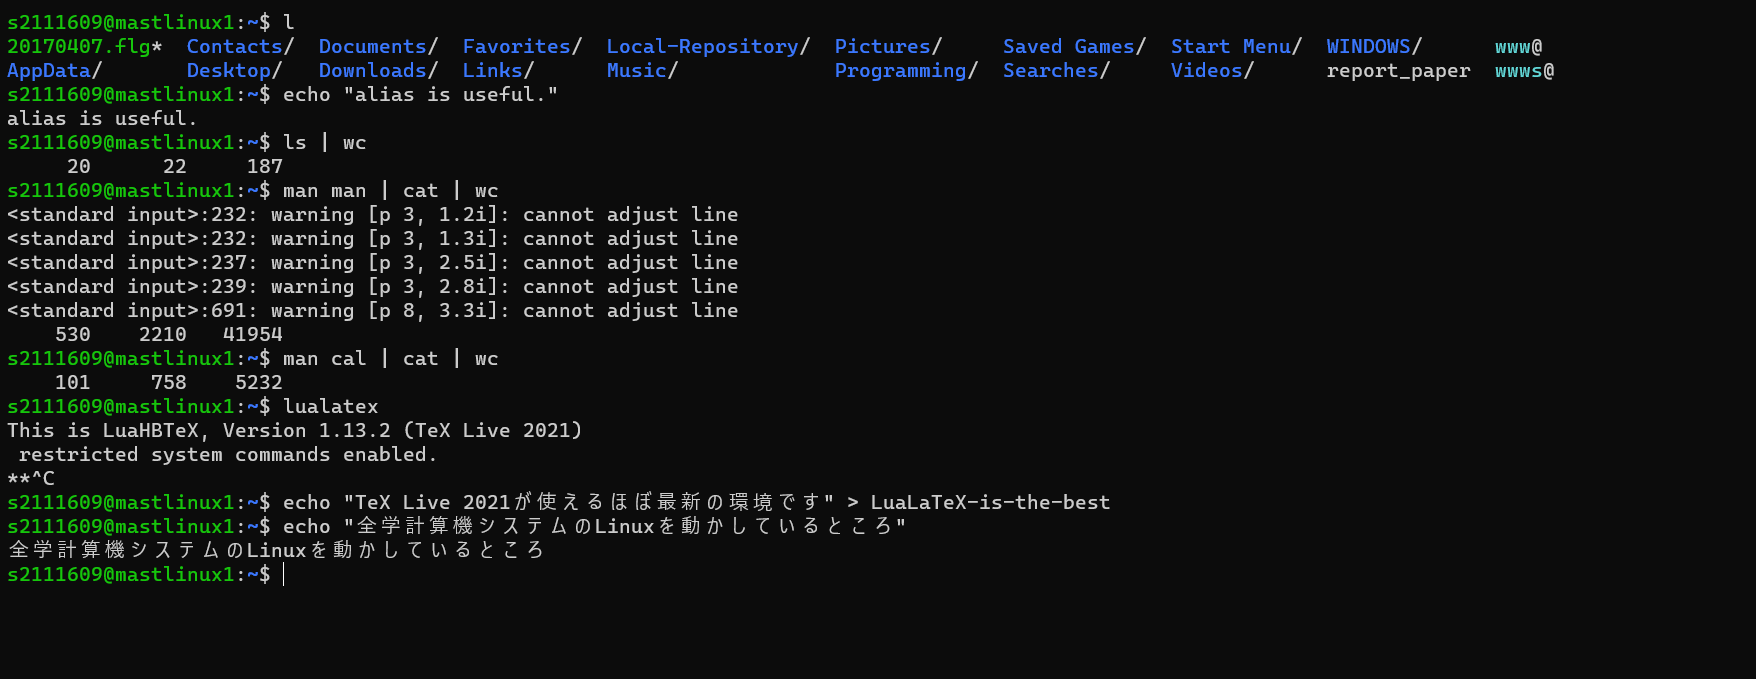
\includegraphics[width=15cm]{imgs/commandline.png}
  \caption{全学計算機を使っているところ}
  \label{fig:keisanki}
\end{figure}

\subsection{確認}
本節の指示内容は次の通りであった。
\begin{enumerate}
  \item キャプチャ方法を含めて、課題内容を達成した方法を記述する \label{enum:how}
  \item 全学計算機システムを利用しているところをキャプチャして図として挿入する\label{enum:figure}
  \item 図の内部で何をしているのかを説明する\label{enum:explain}
\end{enumerate}
\ref{enum:how}は\ref{subsection:方針}節で記述した。\ref{enum:figure}と\ref{enum:explain}は\ref{subsection:実際に挿入する}節で記述した。よって題意を満たしている。
\section{本の紹介}
\subsection{概略}
本節では私の好きな本および、私が世話になった本を紹介したい。私の本棚の本は専門書/技術書が大半を占めているが、それでは面白くないため後半では意図的に技術書ではない本をを2冊紹介することにした。
前半の2冊が世話になった本で後半2冊が好きな本(非技術書)である。
\begin{itemize}
  \item \LaTeXe 美文書作成入門 改訂第8版 ~\cite{bibunsho}
  \item ホログラフィ入門: コンピュータを利用した3次元映像・3次元計測~\cite{holo-nyumon} 
  \item 三日間の幸福~\cite{koufuku}
  \item 恋する小惑星~\cite{koiasu}
\end{itemize}

\subsection{本の内容紹介}
\LaTeXe 美文書作成入門 改訂第8版 ~\cite{bibunsho}は言わずと知れた日本語\LaTeX の大ベストセラー書籍の最新版である。\LaTeX を活用する上で必要なほぼすべてのトピックが網羅されており、日常的に\LaTeX を利用する人は通読したうえで信頼性の高いリファレンスとして手元に置くべき一冊である。

ホログラフィ入門: コンピュータを利用した3次元映像・3次元計測~\cite{holo-nyumon} は私が1年次のAREのときに大変世話になった本であり、ホログラフィの概念、および波動光学を利用した回折計算法などが実装とともに解説されている実用的な一冊である。

三日間の幸福~\cite{koufuku}はWeb発の小説であり、金欠学生の主人公が寿命を売れるという噂を聞き、査定を依頼するが、最低買取価格である1万円/年を言い渡され、生きる気力を失った主人公が残り3カ月を残してすべて売るというシーンから始まる。彼がどのような3カ月を過ごすのか — ぜひ手にとってみてほしい。

恋する小惑星~\cite{koiasu}はまんがタイムきららキャラットに連載された漫画である。「小惑星を見つけたい」という夢を持った高校生の主人公を中心に地質、地図、気象などさまざまな地学の分野に興味をもつ地学系女子たちによる物語である。つくばは本作品の聖地であるから、筑波大学の学生は必見である。
\subsection{確認}
本節での指示内容は以下の通りである。
\begin{itemize}
  \item 課題フォームに記載された構成を満たす
  \item 本をitemize環境で列挙し、文献を参照する
  \item 文献を参照しつつ、100字程度でそれぞれの本の説明を書く
\end{itemize}
本節ではこれらをすべて満たしている。よって設問の題意を満たしていることが確認できた。

\section{感想}
\subsection{Linuxの基礎について}
私はLinuxの利用経験が1年以上あるため、ここまでの講義内容で新たに学んだことや得られたこと、苦労したことはほとんどなかったように思われる。しかし、オプションの類は忘れがちなのでレポートを書く際に改めてそれぞれのコマンドについて調べたことによりいくつか記憶に定着させることができた。また、表としてまとめる際にコマンドのオプションの共通点などが整理できたことは有益だった。(例: -rは再帰的という意味、-iは上書きを防止する、など)

\subsection{\LaTeX について}
私は\LaTeX については昨年少し使ったくらいであり、ローカルで環境構築をして本格的に使い始めたのは今年になってからである。その際にいろいろなことを調べたので講義資料の記述に引っかかりを覚える点が多くあった。正しい知識を得るために\cite{bibunsho}を読み込んだ経験により\LaTeX の知識が大いに向上したことは非常に有意義であった。特にamsmathパッケージ周りの理解が向上したように感じられる。

\subsection{レポートについて}
前節までで記述すべき内容はすべて終了している。ここからはおまけである。

レポートを書くうえで難しかったのは課題内容に対する取り組み方針の記述である。解答を得るための取り組みの手順は書こうと思えばいくらでも細かく書くことができる。今回の出題では求められる高いクオリティの割にテンプレート、例が示されていないのでどれくらいの粒度で書くのが良いとされるのかは全く不明である点が難しかった。

レポートの採点基準についても気になった。課題指示に具体例が示されていないので非常に曖昧な部分が多いように思われる。
\begin{quote}
  上記の注意事項に抵触する場合は、成績評価の範囲
外となる。
\end{quote}

\begin{quote}
  (4) その他の不備は減点の対象となることがある。
\end{quote}
という記述からは教員の一存でどんなレポートでも0点にすることができる権限があると読み取れ、恣意的な運用が可能である。

私個人としては、他人の不備を指摘して減点すると公言するためには、まず自身の資料が完璧であるべきだと考える。時代に即していない内容が堂々と初学者に教えられる現在の状況は大変遺憾である。

\bibliographystyle{junsrt}
\bibliography{citation}
\end{document}
